\documentclass[aspectratio=169,11pt]{beamer}

\usetheme{Madrid}
\usecolortheme{default}
\setbeamertemplate{navigation symbols}{}
\setbeamertemplate{footline}[frame number]

\usepackage{amsmath,amssymb}
\usepackage{graphicx}
\usepackage{tikz}
\usetikzlibrary{positioning,calc}
\usetikzlibrary{arrows.meta,decorations.pathmorphing}

\definecolor{RamRed}{RGB}{190,40,45}
\definecolor{RamBlue}{RGB}{30,90,180}
\definecolor{SoftGray}{RGB}{245,245,245}
\definecolor{DarkGray}{RGB}{70,70,70}
\definecolor{MapGreen}{RGB}{48,150,95}
\definecolor{MapGold}{RGB}{235,180,45}

\setbeamercolor{title}{fg=DarkGray}
\setbeamercolor{frametitle}{fg=white,bg=RamBlue}
\setbeamercolor{structure}{fg=RamBlue}

\tikzset{
  v/.style={circle,draw=black,fill=white,inner sep=1.8pt},
  edge/.style={draw=RamBlue,line width=1.25pt},
  topic/.style={draw=black!30,fill=SoftGray,rounded corners=5pt,inner sep=7pt,
    text width=5.8cm,minimum height=1.65cm,align=left},
}


\usepackage{booktabs}
\tikzset{dot/.style={circle,fill=black,inner sep=2pt}, lab/.style={circle,draw=black,fill=white,inner sep=2pt,minimum size=6mm,font=\small},selected/.style={draw=RamRed,line width=2pt}}
\title{Trails, Circuits, Paths, and Cycles}
\subtitle{Section 1.4 of Harris--Hirst--Mossinghoff}
\author{Jeremy Quastel}
\date{}
\begin{document}
\begin{frame}[plain]{}
\large
\begin{center}{\Huge\bfseries Trails, Circuits,\\[.12cm]Paths, and Cycles}\par\vspace{.25cm}{\Large Section 1.4}\par\vspace{.15cm}{\large Harris--Hirst--Mossinghoff, \emph{Combinatorics and Graph Theory}}\par\vspace{.25cm}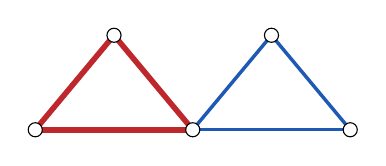
\begin{tikzpicture}[scale=1]
\coordinate (ga) at (-2,0);
\coordinate (gb) at (-1,1.2);
\coordinate (gc) at (0,0);
\coordinate (gd) at (1,1.2);
\coordinate (ge) at (2,0);
\draw[selected] (ga)--(gb);
\draw[selected] (gb)--(gc);
\draw[selected] (gc)--(ga);
\draw[edge] (gc)--(gd);
\draw[edge] (gd)--(ge);
\draw[edge] (ge)--(gc);
\node[v] at (ga) {};
\node[v] at (gb) {};
\node[v] at (gc) {};
\node[v] at (gd) {};
\node[v] at (ge) {};
\end{tikzpicture}\par\vspace{.25cm}Jeremy Quastel\end{center}
\end{frame}

\begin{frame}[plain]{}
\large
\begin{center}{\Huge\bfseries Today's lecture}\par\vspace{.5cm}\end{center}\begin{columns}[c,onlytextwidth]\begin{column}{.48\textwidth}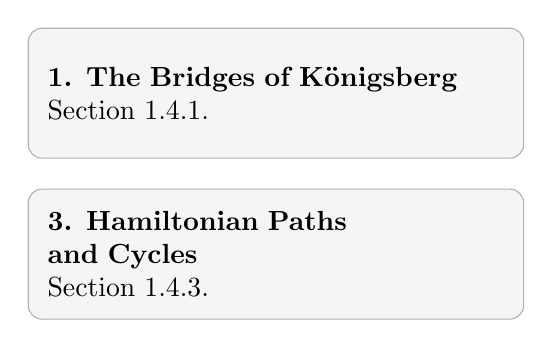
\begin{tikzpicture}\node[topic](a){\textbf{1. The Bridges of K\"onigsberg}\\Section 1.4.1.};\node[topic,below=.38cm of a]{\textbf{3. Hamiltonian Paths\\and Cycles}\\Section 1.4.3.};\end{tikzpicture}\end{column}\begin{column}{.48\textwidth}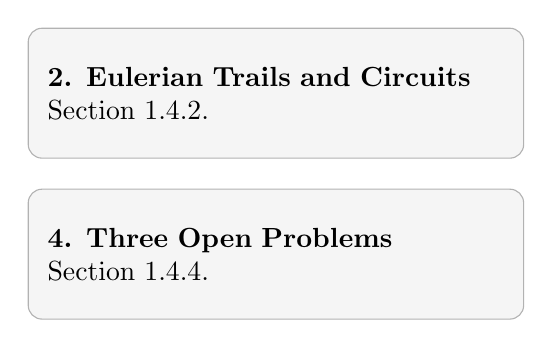
\begin{tikzpicture}\node[topic](a){\textbf{2. Eulerian Trails and Circuits}\\Section 1.4.2.};\node[topic,below=.38cm of a]{\textbf{4. Three Open Problems}\\Section 1.4.4.};\end{tikzpicture}\end{column}\end{columns}
\end{frame}

\begin{frame}{Two Route-Planning Questions}
\large
\begin{block}{Question 1: Covering streets}
Can a route use every street exactly once?
\end{block}
\begin{block}{Question 2: Visiting towns}
Can a route visit every town exactly once?
\end{block}
\bigskip The first question concerns \textbf{edges}; the second concerns \textbf{vertices}.\par\medskip How different can the answers be?
\end{frame}

\begin{frame}{Recall: Walks, Trails, Paths, and Cycles}
\large
\renewcommand{\arraystretch}{1.5}\begin{tabular}{ll}\toprule Walk & Consecutive vertices are adjacent.\\Trail & No edge is repeated.\\Circuit & A closed trail.\\Path & No vertex is repeated.\\Cycle & A closed path, except for the repeated endpoint.\\\bottomrule\end{tabular}\par\bigskip A circuit may revisit a vertex. A cycle cannot revisit a vertex other than its starting vertex at the end.
\end{frame}

\begin{frame}{A Circuit Need Not Be a Cycle}
\large
\begin{center}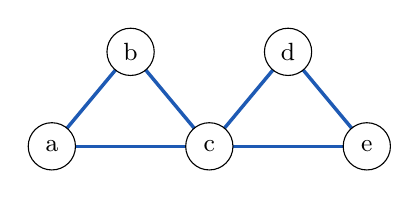
\begin{tikzpicture}[scale=1]
\coordinate (ga) at (-2,0);
\coordinate (gb) at (-1,1.2);
\coordinate (gc) at (0,0);
\coordinate (gd) at (1,1.2);
\coordinate (ge) at (2,0);
\draw[edge] (ga)--(gb);
\draw[edge] (gb)--(gc);
\draw[edge] (gc)--(ga);
\draw[edge] (gc)--(gd);
\draw[edge] (gd)--(ge);
\draw[edge] (ge)--(gc);
\node[lab] at (ga) {a};
\node[lab] at (gb) {b};
\node[lab] at (gc) {c};
\node[lab] at (gd) {d};
\node[lab] at (ge) {e};
\end{tikzpicture}\end{center}\begin{block}{Example}
$a,b,c,d,e,c,a$ is a circuit.\par\smallskip It is not a cycle: the vertex $c$ is visited twice before returning to $a$.
\end{block}

\end{frame}

\section{The Bridges of K\"onigsberg}
\begin{frame}{The Bridges of Königsberg}
\large
\begin{block}{Question}
Can we cross each of the seven bridges exactly once?
\end{block}
\begin{center}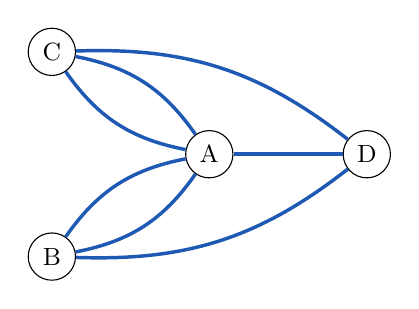
\begin{tikzpicture}[scale=1]
\node[lab](A) at (0,0){A};\node[lab](B) at (-2,-1.3){B};\node[lab](C) at (-2,1.3){C};\node[lab](D) at (2,0){D};
\draw[edge] (A) to[bend left=22] (B);\draw[edge] (A) to[bend right=22] (B);
\draw[edge] (A) to[bend left=22] (C);\draw[edge] (A) to[bend right=22] (C);
\draw[edge] (A)--(D);\draw[edge] (B) to[bend right=20] (D);\draw[edge] (C) to[bend left=20] (D);
\end{tikzpicture}\end{center}Each vertex represents a land mass; each edge represents a bridge.\par\smallskip The route may start and finish at different vertices.
\end{frame}

\begin{frame}{Representing a Route by Letters}
\large
\begin{center}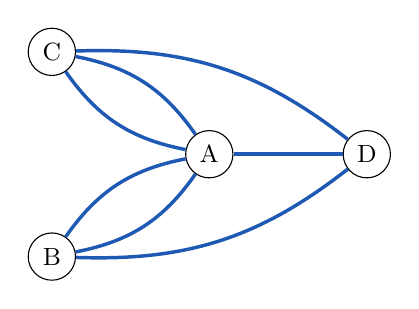
\begin{tikzpicture}[scale=1]
\node[lab](A) at (0,0){A};\node[lab](B) at (-2,-1.3){B};\node[lab](C) at (-2,1.3){C};\node[lab](D) at (2,0){D};
\draw[edge] (A) to[bend left=22] (B);\draw[edge] (A) to[bend right=22] (B);
\draw[edge] (A) to[bend left=22] (C);\draw[edge] (A) to[bend right=22] (C);
\draw[edge] (A)--(D);\draw[edge] (B) to[bend right=20] (D);\draw[edge] (C) to[bend left=20] (D);
\end{tikzpicture}\end{center}The route $A,B,D,A,C,A,B$ uses six bridges.\par\medskip A route crossing all seven bridges would use \textbf{eight letters}.\par\medskip Parallel edges represent different bridges, even when their endpoints agree.
\end{frame}

\begin{frame}{Euler's Counting Idea}
\large
\begin{block}{How many times must each letter appear?}
A vertex with $2k+1$ incident bridges must be an endpoint of the route and must appear $k+1$ times in its letter sequence.
\end{block}
\medskip Here the degrees are $5,3,3,3$. Thus the required occurrences are\[3+2+2+2=9.\]\par But a seven-bridge route has only eight letters.\par\medskip\textbf{No such route exists.}
\end{frame}

\begin{frame}{The Same Obstruction: Odd Degrees}
\large
\begin{block}{Entering and leaving}
At every vertex other than the endpoints, edges used to enter and leave come in pairs.
\end{block}
\begin{center}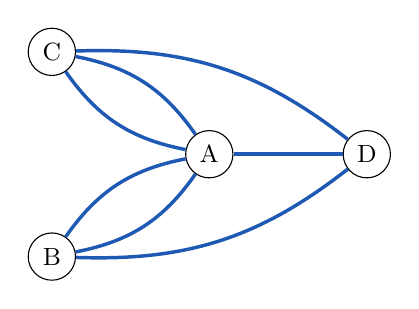
\begin{tikzpicture}[scale=1]
\node[lab](A) at (0,0){A};\node[lab](B) at (-2,-1.3){B};\node[lab](C) at (-2,1.3){C};\node[lab](D) at (2,0){D};
\draw[edge] (A) to[bend left=22] (B);\draw[edge] (A) to[bend right=22] (B);
\draw[edge] (A) to[bend left=22] (C);\draw[edge] (A) to[bend right=22] (C);
\draw[edge] (A)--(D);\draw[edge] (B) to[bend right=20] (D);\draw[edge] (C) to[bend left=20] (D);
\end{tikzpicture}\end{center}There can be at most two vertices of odd degree.\par\smallskip K\"onigsberg has four.
\end{frame}

\begin{frame}{What If We Add One Bridge?}
\large
\begin{center}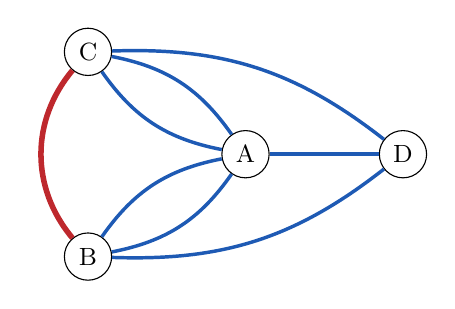
\begin{tikzpicture}[scale=1]
\node[lab](A) at (0,0){A};\node[lab](B) at (-2,-1.3){B};\node[lab](C) at (-2,1.3){C};\node[lab](D) at (2,0){D};
\draw[edge] (A) to[bend left=22] (B);\draw[edge] (A) to[bend right=22] (B);
\draw[edge] (A) to[bend left=22] (C);\draw[edge] (A) to[bend right=22] (C);
\draw[edge] (A)--(D);\draw[edge] (B) to[bend right=20] (D);\draw[edge] (C) to[bend left=20] (D);
\draw[selected] (B) to[bend left=40] (C);\end{tikzpicture}\end{center}\begin{block}{Question}
Add a bridge between $B$ and $C$. Can we now use every bridge exactly once? Where must the route start and end?
\end{block}

\end{frame}

\begin{frame}{What If We Add One Bridge? Answer}
\large
\begin{center}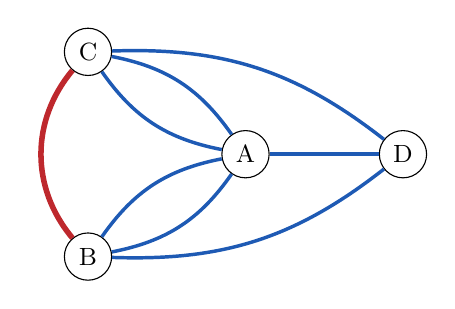
\begin{tikzpicture}[scale=1]
\node[lab](A) at (0,0){A};\node[lab](B) at (-2,-1.3){B};\node[lab](C) at (-2,1.3){C};\node[lab](D) at (2,0){D};
\draw[edge] (A) to[bend left=22] (B);\draw[edge] (A) to[bend right=22] (B);
\draw[edge] (A) to[bend left=22] (C);\draw[edge] (A) to[bend right=22] (C);
\draw[edge] (A)--(D);\draw[edge] (B) to[bend right=20] (D);\draw[edge] (C) to[bend left=20] (D);
\draw[selected] (B) to[bend left=40] (C);\end{tikzpicture}\end{center}Only $A$ and $D$ now have odd degree.\par\medskip One route is\[A,B,A,C,A,D,B,C,D.\]\par The two $AB$ edges and the two $AC$ edges are distinct bridges.
\end{frame}

\section{Eulerian Trails and Circuits}
\begin{frame}{Definition: Eulerian Trails and Circuits}
\large
\begin{block}{Eulerian trail}
A trail using every edge of the graph.
\end{block}
\begin{block}{Eulerian circuit}
A circuit using every edge of the graph.
\end{block}
\begin{block}{Eulerian graph}
A graph containing an Eulerian circuit.
\end{block}
\medskip Vertices may repeat. Edges may not.
\end{frame}

\begin{frame}{Examples: Which Graphs Are Eulerian?}
\large
\begin{columns}[c,onlytextwidth]\begin{column}{.48\textwidth}\begin{center}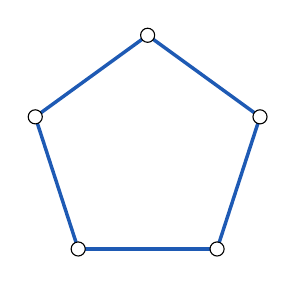
\begin{tikzpicture}[scale=1]
\coordinate (g1) at (0.0,1.5);
\coordinate (g2) at (-1.427,0.464);
\coordinate (g3) at (-0.882,-1.214);
\coordinate (g4) at (0.882,-1.214);
\coordinate (g5) at (1.427,0.464);
\draw[edge] (g1)--(g2);
\draw[edge] (g2)--(g3);
\draw[edge] (g3)--(g4);
\draw[edge] (g4)--(g5);
\draw[edge] (g5)--(g1);
\node[v] at (g1) {};
\node[v] at (g2) {};
\node[v] at (g3) {};
\node[v] at (g4) {};
\node[v] at (g5) {};
\end{tikzpicture}\end{center}\begin{center}$C_5$\end{center}\end{column}\begin{column}{.48\textwidth}\begin{center}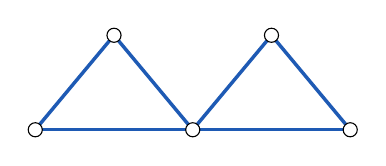
\begin{tikzpicture}[scale=1]
\coordinate (ga) at (-2,0);
\coordinate (gb) at (-1,1.2);
\coordinate (gc) at (0,0);
\coordinate (gd) at (1,1.2);
\coordinate (ge) at (2,0);
\draw[edge] (ga)--(gb);
\draw[edge] (gb)--(gc);
\draw[edge] (gc)--(ga);
\draw[edge] (gc)--(gd);
\draw[edge] (gd)--(ge);
\draw[edge] (ge)--(gc);
\node[v] at (ga) {};
\node[v] at (gb) {};
\node[v] at (gc) {};
\node[v] at (gd) {};
\node[v] at (ge) {};
\end{tikzpicture}\end{center}\begin{center}Two triangles sharing a vertex\end{center}\end{column}\end{columns}\begin{block}{Question}
Does either graph have an Eulerian circuit? Can you describe a route?
\end{block}

\end{frame}

\begin{frame}{Examples: Eulerian Circuits}
\large
\begin{columns}[c,onlytextwidth]\begin{column}{.48\textwidth}\begin{center}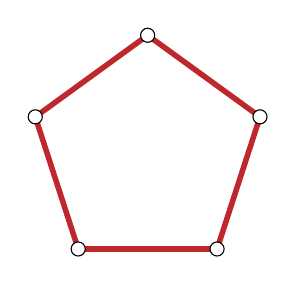
\begin{tikzpicture}[scale=1]
\coordinate (g1) at (0.0,1.5);
\coordinate (g2) at (-1.427,0.464);
\coordinate (g3) at (-0.882,-1.214);
\coordinate (g4) at (0.882,-1.214);
\coordinate (g5) at (1.427,0.464);
\draw[selected] (g1)--(g2);
\draw[selected] (g2)--(g3);
\draw[selected] (g3)--(g4);
\draw[selected] (g4)--(g5);
\draw[selected] (g5)--(g1);
\node[v] at (g1) {};
\node[v] at (g2) {};
\node[v] at (g3) {};
\node[v] at (g4) {};
\node[v] at (g5) {};
\end{tikzpicture}\end{center}\end{column}\begin{column}{.48\textwidth}\begin{center}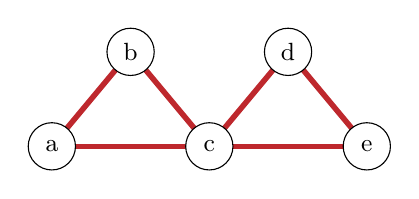
\begin{tikzpicture}[scale=1]
\coordinate (ga) at (-2,0);
\coordinate (gb) at (-1,1.2);
\coordinate (gc) at (0,0);
\coordinate (gd) at (1,1.2);
\coordinate (ge) at (2,0);
\draw[selected] (ga)--(gb);
\draw[selected] (gb)--(gc);
\draw[selected] (gc)--(ga);
\draw[selected] (gc)--(gd);
\draw[selected] (gd)--(ge);
\draw[selected] (ge)--(gc);
\node[lab] at (ga) {a};
\node[lab] at (gb) {b};
\node[lab] at (gc) {c};
\node[lab] at (gd) {d};
\node[lab] at (ge) {e};
\end{tikzpicture}\end{center}\end{column}\end{columns}Both graphs have Eulerian circuits.\par\medskip In the right-hand graph, use $a,b,c,d,e,c,a$.\par\medskip A repeated vertex is allowed in an Eulerian circuit.
\end{frame}

\begin{frame}{Theorem: Characterizing Eulerian Graphs}
\large
\begin{block}{Theorem 1.20}
For a connected graph $G$, the following are equivalent.\begin{enumerate}\item $G$ has an Eulerian circuit.\item Every vertex has even degree.\item $E(G)$ is a disjoint union of edge sets of cycles.\end{enumerate}
\end{block}
\medskip\textbf{Proof plan:} $(1)\Rightarrow(2)\Rightarrow(3)\Rightarrow(1)$.
\end{frame}

\begin{frame}{Proof of Theorem 1.20: Even Degrees}
\large
\begin{block}{Recall}
An Eulerian circuit forces all degrees to be even.
\end{block}
\begin{block}{Proof}
\normalsize Follow the circuit from its starting vertex. Each arrival is paired with a departure, using two distinct edges. At the starting vertex, pair the first departure with the final arrival.\par\medskip Every incident edge is used exactly once, so the degree of every vertex is even.\hfill$\square$
\end{block}

\end{frame}

\begin{frame}{Proof Continued: Partitioning into Cycles}
\large
\begin{block}{Recall}
If all degrees are even, the edges can be partitioned into cycles.
\end{block}
\begin{block}{Proof}
\normalsize If edges remain, some nontrivial component has minimum degree at least $2$, so it contains a cycle $S$. Remove the edges of $S$.\par\medskip Each vertex of $S$ loses two incident edges; every degree remains even. Repeat on the remaining graph.\par\medskip The number of edges decreases, so the procedure ends. The removed cycles partition the original edge set.\hfill$\square$
\end{block}
\small Isolated vertices contribute no edges; the empty edge set has the empty partition.
\end{frame}

\begin{frame}{Partitioning into Cycles: Example}
\large
\begin{center}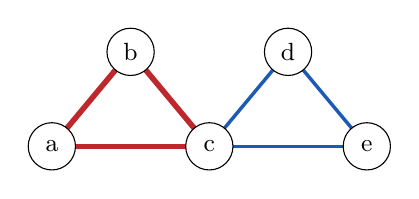
\begin{tikzpicture}[scale=1]
\coordinate (ga) at (-2,0);
\coordinate (gb) at (-1,1.2);
\coordinate (gc) at (0,0);
\coordinate (gd) at (1,1.2);
\coordinate (ge) at (2,0);
\draw[selected] (ga)--(gb);
\draw[selected] (gb)--(gc);
\draw[selected] (gc)--(ga);
\draw[edge] (gc)--(gd);
\draw[edge] (gd)--(ge);
\draw[edge] (ge)--(gc);
\node[lab] at (ga) {a};
\node[lab] at (gb) {b};
\node[lab] at (gc) {c};
\node[lab] at (gd) {d};
\node[lab] at (ge) {e};
\end{tikzpicture}\end{center}The red triangle and the blue triangle have disjoint edge sets.\par\medskip They share the vertex $c$, which is allowed.\par\medskip Removing the red cycle changes the degree of $c$ from $4$ to $2$.
\end{frame}

\begin{frame}{Proof Continued: Joining the Cycles}
\large
\begin{block}{Recall}
An edge partition into cycles gives an Eulerian circuit.
\end{block}
\begin{block}{Proof}
\normalsize Choose a circuit $C$ using the edges of as many whole cycles of the partition as possible.\par\medskip If an edge remains unused, connectedness gives an unused edge incident with a vertex $v$ of $C$. The partition cycle $S$ containing that edge is entirely unused.\par\medskip At $v$, traverse $S$, return to $v$, and then continue around $C$. This is a larger circuit, a contradiction.\hfill$\square$
\end{block}

\end{frame}

\begin{frame}{Joining Two Circuits}
\large
\begin{center}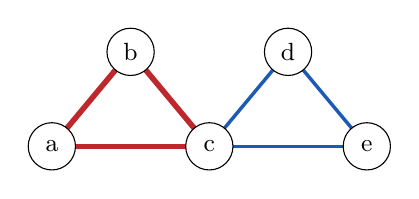
\begin{tikzpicture}[scale=1]
\coordinate (ga) at (-2,0);
\coordinate (gb) at (-1,1.2);
\coordinate (gc) at (0,0);
\coordinate (gd) at (1,1.2);
\coordinate (ge) at (2,0);
\draw[selected] (ga)--(gb);
\draw[selected] (gb)--(gc);
\draw[selected] (gc)--(ga);
\draw[edge] (gc)--(gd);
\draw[edge] (gd)--(ge);
\draw[edge] (ge)--(gc);
\node[lab] at (ga) {a};
\node[lab] at (gb) {b};
\node[lab] at (gc) {c};
\node[lab] at (gd) {d};
\node[lab] at (ge) {e};
\end{tikzpicture}\end{center}Start with $a,b,c,a$. Insert $c,d,e,c$ at $c$:\[a,b,\underbrace{c,d,e,c}_{\text{inserted circuit}},a.\]\par No edge is repeated, because the two circuits have disjoint edge sets.
\end{frame}

\begin{frame}{Corollary: Eulerian Trails}
\large
\begin{block}{Corollary 1.21}
A connected graph has an Eulerian trail exactly when it has at most two vertices of odd degree.
\end{block}
\begin{itemize}\setlength{\itemsep}{.22cm}
\item No odd-degree vertices: the route can be closed.
\item Exactly two odd-degree vertices: they are the endpoints.
\item More than two odd-degree vertices: no Eulerian trail.
\end{itemize}\medskip Recall: the number of odd-degree vertices is always even.
\end{frame}

\begin{frame}{Proof of Corollary 1.21}
\large
\begin{block}{Recall}
A connected graph has an Eulerian trail iff it has $0$ or $2$ odd-degree vertices.
\end{block}
\begin{block}{Proof}
\normalsize \textbf{Necessity.} Pair arrivals and departures at all internal vertices. Only the two endpoints can have odd degree.\par\medskip\textbf{Sufficiency.} With no odd degrees, use Theorem 1.20. With odd vertices $u,v$, add a new vertex $x$ and edges $ux,xv$. All degrees are now even.\par\medskip Take an Eulerian circuit and remove the segment $u,x,v$. The remaining route is an Eulerian trail from $v$ to $u$.\hfill$\square$
\end{block}

\end{frame}

\begin{frame}{Hierholzer's Algorithm}
\large
Once we know an Eulerian circuit exists, how do we find one?\begin{block}{Algorithm}
\begin{enumerate}\item Build a circuit and mark its edges.\item If all edges are marked, stop.\item Choose a vertex on the circuit incident with an unmarked edge.\item From that vertex, build a circuit using unmarked edges.\item Insert the new circuit into the old one and repeat.\end{enumerate}
\end{block}

\end{frame}

\begin{frame}{Hierholzer's Algorithm: Step 1}
\large
\begin{columns}[c,onlytextwidth]\begin{column}{.48\textwidth}\begin{center}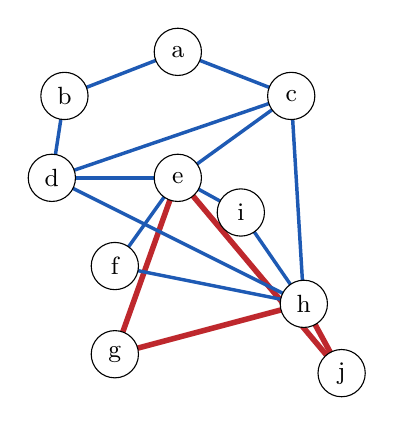
\begin{tikzpicture}[scale=0.8]
\coordinate (ga) at (0,2);
\coordinate (gb) at (-1.8,1.3);
\coordinate (gc) at (1.8,1.3);
\coordinate (gd) at (-2,0);
\coordinate (ge) at (0,0);
\coordinate (gf) at (-1,-1.4);
\coordinate (gg) at (-1,-2.8);
\coordinate (gh) at (2,-2);
\coordinate (gi) at (1,-0.55);
\coordinate (gj) at (2.6,-3.1);
\draw[selected] (ge)--(gg);
\draw[selected] (gg)--(gh);
\draw[selected] (gh)--(gj);
\draw[selected] (gj)--(ge);
\draw[edge] (gh)--(gd);
\draw[edge] (gd)--(gc);
\draw[edge] (gc)--(gh);
\draw[edge] (gd)--(gb);
\draw[edge] (gb)--(ga);
\draw[edge] (ga)--(gc);
\draw[edge] (gc)--(ge);
\draw[edge] (ge)--(gd);
\draw[edge] (gh)--(gf);
\draw[edge] (gf)--(ge);
\draw[edge] (ge)--(gi);
\draw[edge] (gi)--(gh);
\node[lab] at (ga) {a};
\node[lab] at (gb) {b};
\node[lab] at (gc) {c};
\node[lab] at (gd) {d};
\node[lab] at (ge) {e};
\node[lab] at (gf) {f};
\node[lab] at (gg) {g};
\node[lab] at (gh) {h};
\node[lab] at (gi) {i};
\node[lab] at (gj) {j};
\end{tikzpicture}\end{center}\end{column}\begin{column}{.48\textwidth}Choose $R_1=e,g,h,j,e$.\begin{block}{Current circuit}
\normalsize $R_1=e,g,h,j,e.$
\end{block}
Red edges have been used. Blue edges remain.\end{column}\end{columns}
\end{frame}

\begin{frame}{Hierholzer's Algorithm: Step 2}
\large
\begin{columns}[c,onlytextwidth]\begin{column}{.48\textwidth}\begin{center}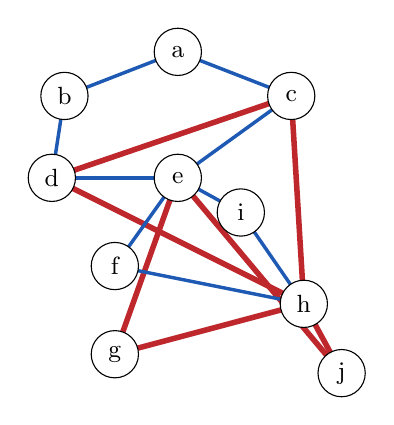
\begin{tikzpicture}[scale=0.8]
\coordinate (ga) at (0,2);
\coordinate (gb) at (-1.8,1.3);
\coordinate (gc) at (1.8,1.3);
\coordinate (gd) at (-2,0);
\coordinate (ge) at (0,0);
\coordinate (gf) at (-1,-1.4);
\coordinate (gg) at (-1,-2.8);
\coordinate (gh) at (2,-2);
\coordinate (gi) at (1,-0.55);
\coordinate (gj) at (2.6,-3.1);
\draw[selected] (ge)--(gg);
\draw[selected] (gg)--(gh);
\draw[selected] (gh)--(gj);
\draw[selected] (gj)--(ge);
\draw[selected] (gh)--(gd);
\draw[selected] (gd)--(gc);
\draw[selected] (gc)--(gh);
\draw[edge] (gd)--(gb);
\draw[edge] (gb)--(ga);
\draw[edge] (ga)--(gc);
\draw[edge] (gc)--(ge);
\draw[edge] (ge)--(gd);
\draw[edge] (gh)--(gf);
\draw[edge] (gf)--(ge);
\draw[edge] (ge)--(gi);
\draw[edge] (gi)--(gh);
\node[lab] at (ga) {a};
\node[lab] at (gb) {b};
\node[lab] at (gc) {c};
\node[lab] at (gd) {d};
\node[lab] at (ge) {e};
\node[lab] at (gf) {f};
\node[lab] at (gg) {g};
\node[lab] at (gh) {h};
\node[lab] at (gi) {i};
\node[lab] at (gj) {j};
\end{tikzpicture}\end{center}\end{column}\begin{column}{.48\textwidth}At $h$, insert $Q_1=h,d,c,h$.\begin{block}{Current circuit}
\normalsize $R_2=e,g,h,d,c,h,j,e.$
\end{block}
Red edges have been used. Blue edges remain.\end{column}\end{columns}
\end{frame}

\begin{frame}{Hierholzer's Algorithm: Step 3}
\large
\begin{columns}[c,onlytextwidth]\begin{column}{.48\textwidth}\begin{center}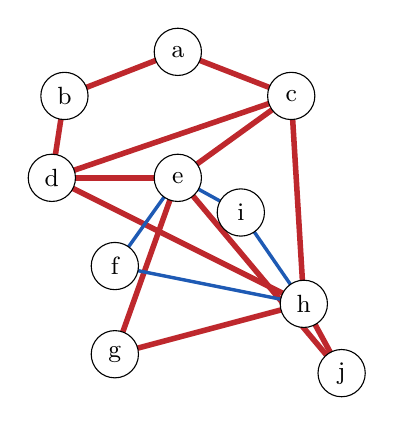
\begin{tikzpicture}[scale=0.8]
\coordinate (ga) at (0,2);
\coordinate (gb) at (-1.8,1.3);
\coordinate (gc) at (1.8,1.3);
\coordinate (gd) at (-2,0);
\coordinate (ge) at (0,0);
\coordinate (gf) at (-1,-1.4);
\coordinate (gg) at (-1,-2.8);
\coordinate (gh) at (2,-2);
\coordinate (gi) at (1,-0.55);
\coordinate (gj) at (2.6,-3.1);
\draw[selected] (ge)--(gg);
\draw[selected] (gg)--(gh);
\draw[selected] (gh)--(gj);
\draw[selected] (gj)--(ge);
\draw[selected] (gh)--(gd);
\draw[selected] (gd)--(gc);
\draw[selected] (gc)--(gh);
\draw[selected] (gd)--(gb);
\draw[selected] (gb)--(ga);
\draw[selected] (ga)--(gc);
\draw[selected] (gc)--(ge);
\draw[selected] (ge)--(gd);
\draw[edge] (gh)--(gf);
\draw[edge] (gf)--(ge);
\draw[edge] (ge)--(gi);
\draw[edge] (gi)--(gh);
\node[lab] at (ga) {a};
\node[lab] at (gb) {b};
\node[lab] at (gc) {c};
\node[lab] at (gd) {d};
\node[lab] at (ge) {e};
\node[lab] at (gf) {f};
\node[lab] at (gg) {g};
\node[lab] at (gh) {h};
\node[lab] at (gi) {i};
\node[lab] at (gj) {j};
\end{tikzpicture}\end{center}\end{column}\begin{column}{.48\textwidth}At $d$, insert $Q_2=d,b,a,c,e,d$.\begin{block}{Current circuit}
\normalsize $R_3=e,g,h,d,b,a,c,e,d,c,h,j,e.$
\end{block}
Red edges have been used. Blue edges remain.\end{column}\end{columns}
\end{frame}

\begin{frame}{Hierholzer's Algorithm: Step 4}
\large
\begin{columns}[c,onlytextwidth]\begin{column}{.48\textwidth}\begin{center}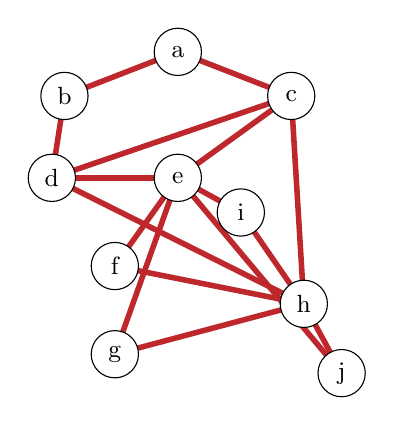
\begin{tikzpicture}[scale=0.8]
\coordinate (ga) at (0,2);
\coordinate (gb) at (-1.8,1.3);
\coordinate (gc) at (1.8,1.3);
\coordinate (gd) at (-2,0);
\coordinate (ge) at (0,0);
\coordinate (gf) at (-1,-1.4);
\coordinate (gg) at (-1,-2.8);
\coordinate (gh) at (2,-2);
\coordinate (gi) at (1,-0.55);
\coordinate (gj) at (2.6,-3.1);
\draw[selected] (ge)--(gg);
\draw[selected] (gg)--(gh);
\draw[selected] (gh)--(gj);
\draw[selected] (gj)--(ge);
\draw[selected] (gh)--(gd);
\draw[selected] (gd)--(gc);
\draw[selected] (gc)--(gh);
\draw[selected] (gd)--(gb);
\draw[selected] (gb)--(ga);
\draw[selected] (ga)--(gc);
\draw[selected] (gc)--(ge);
\draw[selected] (ge)--(gd);
\draw[selected] (gh)--(gf);
\draw[selected] (gf)--(ge);
\draw[selected] (ge)--(gi);
\draw[selected] (gi)--(gh);
\node[lab] at (ga) {a};
\node[lab] at (gb) {b};
\node[lab] at (gc) {c};
\node[lab] at (gd) {d};
\node[lab] at (ge) {e};
\node[lab] at (gf) {f};
\node[lab] at (gg) {g};
\node[lab] at (gh) {h};
\node[lab] at (gi) {i};
\node[lab] at (gj) {j};
\end{tikzpicture}\end{center}\end{column}\begin{column}{.48\textwidth}At $h$, insert $Q_3=h,f,e,i,h$.\begin{block}{Current circuit}
\normalsize $R_4=e,g,h,f,e,i,h,d,b,a,c,e,d,c,h,j,e.$
\end{block}
All $16$ edges are now used.\end{column}\end{columns}
\end{frame}

\begin{frame}{Why Hierholzer's Algorithm Works}
\large
\begin{itemize}\setlength{\itemsep}{.22cm}
\item Removing a circuit leaves every remaining degree even.
\item A trail following unused edges can get stuck only at its starting vertex; this produces another circuit.
\item If unused edges remain, connectedness gives a place to attach another circuit.
\item Each insertion adds edges. Since the graph is finite, the algorithm stops.
\end{itemize}
\end{frame}

\section{Hamiltonian Paths and Cycles}
\begin{frame}{From Edges to Vertices}
\large
\begin{block}{A different question}
Can we visit every vertex exactly once, and return to the start?
\end{block}
\medskip Hamilton\textquotesingle s Icosian game asks for such a route on the graph of a dodecahedron.\par\medskip We now seek a \textbf{spanning cycle}, rather than a circuit using every edge.
\end{frame}

\begin{frame}{The Icosian Game}
\large
\begin{columns}[c,onlytextwidth]\begin{column}{.48\textwidth}\begin{center}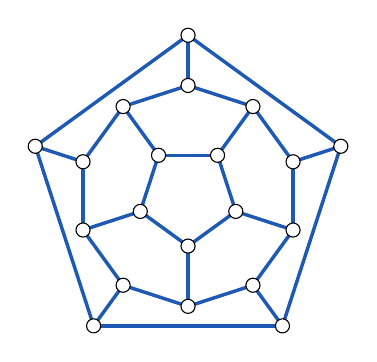
\begin{tikzpicture}[scale=0.85]
\coordinate (g0) at (1.4695761589768238e-16,2.4);
\coordinate (g1) at (-2.282535639108368,0.741640786499874);
\coordinate (g2) at (-1.4106846055019358,-1.9416407864998735);
\coordinate (g3) at (1.4106846055019349,-1.9416407864998741);
\coordinate (g4) at (2.2825356391083687,0.7416407864998732);
\coordinate (g5) at (1.0103336092965664e-16,1.65);
\coordinate (g6) at (-0.9698456662825804,1.3348780407186631);
\coordinate (g7) at (-1.5692432518870032,0.5098780407186634);
\coordinate (g8) at (-1.5692432518870034,-0.5098780407186629);
\coordinate (g9) at (-0.9698456662825808,-1.3348780407186631);
\coordinate (g10) at (-3.031000827889699e-16,-1.65);
\coordinate (g11) at (0.9698456662825803,-1.3348780407186633);
\coordinate (g12) at (1.5692432518870032,-0.5098780407186635);
\coordinate (g13) at (1.5692432518870034,0.5098780407186628);
\coordinate (g14) at (0.969845666282581,1.334878040718663);
\coordinate (g15) at (-0.4408389392193548,0.6067627457812106);
\coordinate (g16) at (-0.7132923872213652,-0.23176274578121048);
\coordinate (g17) at (-1.3777276490407724e-16,-0.75);
\coordinate (g18) at (0.7132923872213651,-0.2317627457812107);
\coordinate (g19) at (0.440838939219355,0.6067627457812104);
\draw[edge] (g0)--(g1);
\draw[edge] (g1)--(g2);
\draw[edge] (g2)--(g3);
\draw[edge] (g3)--(g4);
\draw[edge] (g4)--(g0);
\draw[edge] (g5)--(g6);
\draw[edge] (g6)--(g7);
\draw[edge] (g7)--(g8);
\draw[edge] (g8)--(g9);
\draw[edge] (g9)--(g10);
\draw[edge] (g10)--(g11);
\draw[edge] (g11)--(g12);
\draw[edge] (g12)--(g13);
\draw[edge] (g13)--(g14);
\draw[edge] (g14)--(g5);
\draw[edge] (g15)--(g16);
\draw[edge] (g16)--(g17);
\draw[edge] (g17)--(g18);
\draw[edge] (g18)--(g19);
\draw[edge] (g19)--(g15);
\draw[edge] (g0)--(g5);
\draw[edge] (g1)--(g7);
\draw[edge] (g2)--(g9);
\draw[edge] (g3)--(g11);
\draw[edge] (g4)--(g13);
\draw[edge] (g15)--(g6);
\draw[edge] (g16)--(g8);
\draw[edge] (g17)--(g10);
\draw[edge] (g18)--(g12);
\draw[edge] (g19)--(g14);
\node[v] at (g0) {};
\node[v] at (g1) {};
\node[v] at (g2) {};
\node[v] at (g3) {};
\node[v] at (g4) {};
\node[v] at (g5) {};
\node[v] at (g6) {};
\node[v] at (g7) {};
\node[v] at (g8) {};
\node[v] at (g9) {};
\node[v] at (g10) {};
\node[v] at (g11) {};
\node[v] at (g12) {};
\node[v] at (g13) {};
\node[v] at (g14) {};
\node[v] at (g15) {};
\node[v] at (g16) {};
\node[v] at (g17) {};
\node[v] at (g18) {};
\node[v] at (g19) {};
\end{tikzpicture}\end{center}\end{column}\begin{column}{.48\textwidth}\begin{block}{Question}
Find a cycle through all twenty vertices of the dodecahedral graph.
\end{block}
\medskip The drawing has been flattened into the plane. Adjacencies remain the same.\end{column}\end{columns}
\end{frame}

\begin{frame}{The Icosian Game: A Solution}
\large
\begin{columns}[c,onlytextwidth]\begin{column}{.48\textwidth}\begin{center}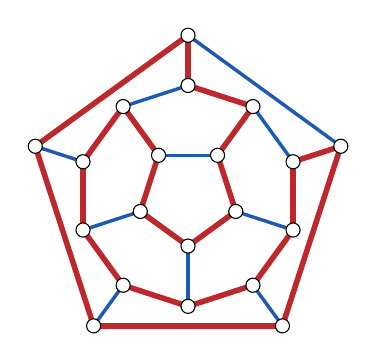
\begin{tikzpicture}[scale=0.85]
\coordinate (g0) at (1.4695761589768238e-16,2.4);
\coordinate (g1) at (-2.282535639108368,0.741640786499874);
\coordinate (g2) at (-1.4106846055019358,-1.9416407864998735);
\coordinate (g3) at (1.4106846055019349,-1.9416407864998741);
\coordinate (g4) at (2.2825356391083687,0.7416407864998732);
\coordinate (g5) at (1.0103336092965664e-16,1.65);
\coordinate (g6) at (-0.9698456662825804,1.3348780407186631);
\coordinate (g7) at (-1.5692432518870032,0.5098780407186634);
\coordinate (g8) at (-1.5692432518870034,-0.5098780407186629);
\coordinate (g9) at (-0.9698456662825808,-1.3348780407186631);
\coordinate (g10) at (-3.031000827889699e-16,-1.65);
\coordinate (g11) at (0.9698456662825803,-1.3348780407186633);
\coordinate (g12) at (1.5692432518870032,-0.5098780407186635);
\coordinate (g13) at (1.5692432518870034,0.5098780407186628);
\coordinate (g14) at (0.969845666282581,1.334878040718663);
\coordinate (g15) at (-0.4408389392193548,0.6067627457812106);
\coordinate (g16) at (-0.7132923872213652,-0.23176274578121048);
\coordinate (g17) at (-1.3777276490407724e-16,-0.75);
\coordinate (g18) at (0.7132923872213651,-0.2317627457812107);
\coordinate (g19) at (0.440838939219355,0.6067627457812104);
\draw[selected] (g0)--(g1);
\draw[selected] (g1)--(g2);
\draw[selected] (g2)--(g3);
\draw[selected] (g3)--(g4);
\draw[edge] (g4)--(g0);
\draw[edge] (g5)--(g6);
\draw[selected] (g6)--(g7);
\draw[selected] (g7)--(g8);
\draw[selected] (g8)--(g9);
\draw[selected] (g9)--(g10);
\draw[selected] (g10)--(g11);
\draw[selected] (g11)--(g12);
\draw[selected] (g12)--(g13);
\draw[edge] (g13)--(g14);
\draw[selected] (g14)--(g5);
\draw[selected] (g15)--(g16);
\draw[selected] (g16)--(g17);
\draw[selected] (g17)--(g18);
\draw[selected] (g18)--(g19);
\draw[edge] (g19)--(g15);
\draw[selected] (g0)--(g5);
\draw[edge] (g1)--(g7);
\draw[edge] (g2)--(g9);
\draw[edge] (g3)--(g11);
\draw[selected] (g4)--(g13);
\draw[selected] (g15)--(g6);
\draw[edge] (g16)--(g8);
\draw[edge] (g17)--(g10);
\draw[edge] (g18)--(g12);
\draw[selected] (g19)--(g14);
\node[v] at (g0) {};
\node[v] at (g1) {};
\node[v] at (g2) {};
\node[v] at (g3) {};
\node[v] at (g4) {};
\node[v] at (g5) {};
\node[v] at (g6) {};
\node[v] at (g7) {};
\node[v] at (g8) {};
\node[v] at (g9) {};
\node[v] at (g10) {};
\node[v] at (g11) {};
\node[v] at (g12) {};
\node[v] at (g13) {};
\node[v] at (g14) {};
\node[v] at (g15) {};
\node[v] at (g16) {};
\node[v] at (g17) {};
\node[v] at (g18) {};
\node[v] at (g19) {};
\end{tikzpicture}\end{center}\end{column}\begin{column}{.48\textwidth}The red cycle visits each vertex exactly once before returning to the start.\par\medskip It uses $20$ of the graph's $30$ edges.\par\medskip This is the type of route we call Hamiltonian.\end{column}\end{columns}
\end{frame}

\begin{frame}{Definition: Hamiltonian Paths and Cycles}
\large
\begin{block}{Hamiltonian path and traceable graph}
A Hamiltonian path contains every vertex. A graph with such a path is called traceable.
\end{block}
\begin{block}{Hamiltonian cycle and Hamiltonian graph}
A Hamiltonian cycle contains every vertex. A graph with such a cycle is called Hamiltonian.
\end{block}
\medskip Every Hamiltonian graph is traceable: remove one edge of its spanning cycle.
\end{frame}

\begin{frame}{Examples: Hamiltonian, Traceable, or Neither?}
\large
\begin{columns}[c,onlytextwidth]\begin{column}{.48\textwidth}\begin{center}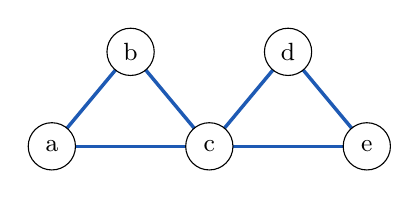
\begin{tikzpicture}[scale=1]
\coordinate (ga) at (-2,0);
\coordinate (gb) at (-1,1.2);
\coordinate (gc) at (0,0);
\coordinate (gd) at (1,1.2);
\coordinate (ge) at (2,0);
\draw[edge] (ga)--(gb);
\draw[edge] (gb)--(gc);
\draw[edge] (gc)--(ga);
\draw[edge] (gc)--(gd);
\draw[edge] (gd)--(ge);
\draw[edge] (ge)--(gc);
\node[lab] at (ga) {a};
\node[lab] at (gb) {b};
\node[lab] at (gc) {c};
\node[lab] at (gd) {d};
\node[lab] at (ge) {e};
\end{tikzpicture}\end{center}\begin{center}Two triangles sharing a vertex\end{center}\end{column}\begin{column}{.48\textwidth}\begin{center}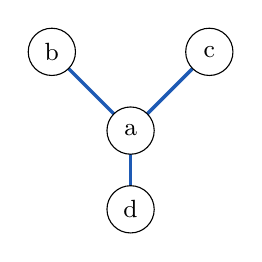
\begin{tikzpicture}[scale=1]
\coordinate (ga) at (0,0);
\coordinate (gb) at (-1,1);
\coordinate (gc) at (1,1);
\coordinate (gd) at (0,-1);
\draw[edge] (ga)--(gb);
\draw[edge] (ga)--(gc);
\draw[edge] (ga)--(gd);
\node[lab] at (ga) {a};
\node[lab] at (gb) {b};
\node[lab] at (gc) {c};
\node[lab] at (gd) {d};
\end{tikzpicture}\end{center}\end{column}\end{columns}\begin{block}{Question}
Which graphs have spanning paths? Which have spanning cycles?
\end{block}

\end{frame}

\begin{frame}{Examples: Answers}
\large
\begin{columns}[c,onlytextwidth]\begin{column}{.48\textwidth}\begin{center}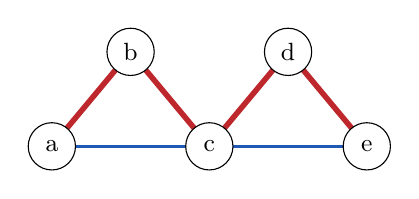
\begin{tikzpicture}[scale=1]
\coordinate (ga) at (-2,0);
\coordinate (gb) at (-1,1.2);
\coordinate (gc) at (0,0);
\coordinate (gd) at (1,1.2);
\coordinate (ge) at (2,0);
\draw[selected] (ga)--(gb);
\draw[selected] (gb)--(gc);
\draw[edge] (gc)--(ga);
\draw[selected] (gc)--(gd);
\draw[selected] (gd)--(ge);
\draw[edge] (ge)--(gc);
\node[lab] at (ga) {a};
\node[lab] at (gb) {b};
\node[lab] at (gc) {c};
\node[lab] at (gd) {d};
\node[lab] at (ge) {e};
\end{tikzpicture}\end{center}\end{column}\begin{column}{.48\textwidth}\begin{center}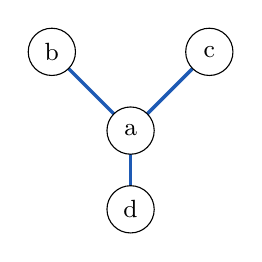
\begin{tikzpicture}[scale=1]
\coordinate (ga) at (0,0);
\coordinate (gb) at (-1,1);
\coordinate (gc) at (1,1);
\coordinate (gd) at (0,-1);
\draw[edge] (ga)--(gb);
\draw[edge] (ga)--(gc);
\draw[edge] (ga)--(gd);
\node[lab] at (ga) {a};
\node[lab] at (gb) {b};
\node[lab] at (gc) {c};
\node[lab] at (gd) {d};
\end{tikzpicture}\end{center}\end{column}\end{columns}\textbf{Left:} traceable via $a,b,c,d,e$, but not Hamiltonian. A cycle cannot visit both triangles without repeating $c$.\par\medskip\textbf{Right:} neither. A spanning path would need all three leaves as endpoints.
\end{frame}

\begin{frame}{Eulerian and Hamiltonian Are Different}
\large
\renewcommand{\arraystretch}{1.5}\begin{tabular}{lcc}\toprule Graph & Eulerian? & Hamiltonian?\\\midrule $C_5$ & Yes & Yes\\Two triangles sharing a vertex & Yes & No\\$K_4$ & No & Yes\\$P_4$ & No & No\\\bottomrule\end{tabular}\par\bigskip Degree parity completely determines Eulerian circuits in connected graphs. It does not determine Hamiltonian cycles.
\end{frame}

\begin{frame}{Hamiltonian Graphs Must Be 2-Connected}
\large
\begin{block}{Observation}
If $G$ is Hamiltonian, then deleting any one vertex leaves a connected graph.
\end{block}
\medskip Delete a vertex from a Hamiltonian cycle. The remaining edges of the cycle form a path through all remaining vertices.\par\bigskip Thus a cut vertex rules out Hamiltonicity.\par\medskip The reverse implication is false.
\end{frame}

\begin{frame}{Theorem: Dirac's Theorem}
\large
\begin{block}{Theorem 1.22}
For a graph of order $n\ge3$, $\delta(G)\ge n/2$ implies that $G$ is Hamiltonian.
\end{block}
\bigskip Large degrees can force a spanning cycle.\par\medskip We prove this by turning a longest path into a cycle.
\end{frame}

\begin{frame}{Proof of Dirac's Theorem: A Longest Path}
\large
\begin{block}{Recall}
For a graph of order $n\ge3$, $\delta(G)\ge n/2$ implies that $G$ is Hamiltonian.
\end{block}
\begin{block}{Proof}
\normalsize First, $G$ is connected: each component has at least $\delta(G)+1>n/2$ vertices, so two components are impossible.\par\medskip Choose a longest path $P=v_1,v_2,\ldots,v_p$. Every neighbor of either endpoint lies on $P$; otherwise the path could be extended.
\end{block}

\end{frame}

\begin{frame}{Proof Continued: Finding Two Cross Edges}
\large
\begin{block}{Recall}
$P=v_1,\ldots,v_p$ is a longest path.
\end{block}
\begin{block}{Proof}
\normalsize In $\{1,\ldots,p-1\}$, define\[A=\{i:v_1v_{i+1}\in E(G)\},\qquad B=\{i:v_iv_p\in E(G)\}.\]All endpoint neighbors lie on $P$, so\[|A|+|B|=\deg(v_1)+\deg(v_p)\ge n>p-1.\]Thus $A\cap B\ne\varnothing$. For some $j$, both $v_1v_{j+1}$ and $v_jv_p$ are edges.
\end{block}

\end{frame}

\begin{frame}{Proof Continued: Closing the Path}
\large
\begin{center}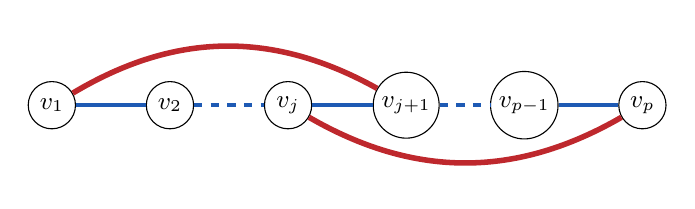
\begin{tikzpicture}[x=1.5cm]\foreach \i/\t in {1/v_1,2/v_2,3/v_j,4/v_{j+1},5/v_{p-1},6/v_p}{\node[lab](p\i) at (\i,0){$\t$};}\draw[edge](p1)--(p2);\draw[edge,dashed](p2)--(p3);\draw[edge](p3)--(p4);\draw[edge,dashed](p4)--(p5);\draw[edge](p5)--(p6);\draw[selected](p1) to[bend left=30](p4);\draw[selected](p3) to[bend right=30](p6);\end{tikzpicture}\end{center}\bigskip Follow the vertices in this order:\[v_1,v_2,\ldots,v_j,v_p,v_{p-1},\ldots,v_{j+1},v_1.\]\par This is a cycle containing every vertex of $P$.
\end{frame}

\begin{frame}{Proof Continued: The Cycle Is Spanning}
\large
\begin{block}{Recall}
There is a cycle $C$ containing every vertex of a longest path $P$.
\end{block}
\begin{block}{Proof}
\normalsize If $C$ misses a vertex, connectedness gives an edge $xy$ with $x\notin V(C)$ and $y\in V(C)$.\par\medskip Start at $x$, move to $y$, and follow $C$ without closing it. This gives a path with $p+1$ vertices, contradicting the choice of $P$.\par\medskip Hence $p=n$, and $C$ is Hamiltonian.\hfill$\square$
\end{block}

\end{frame}

\begin{frame}{Dirac's Bound: Sharp, but Not Necessary}
\large
\begin{block}{Sharpness}
$K_{r,r+1}$ has $n=2r+1$ and minimum degree $r=(n-1)/2$. It has no Hamiltonian cycle: a cycle in a bipartite graph uses equal numbers of vertices from the two parts.
\end{block}
\begin{block}{Not a characterization}
For $n\ge5$, the graph $C_n$ is Hamiltonian but has minimum degree $2<n/2$.
\end{block}

\end{frame}

\begin{frame}{Theorem: Ore's Theorem}
\large
\begin{block}{Theorem 1.23}
Let $|V(G)|=n\ge3$. If\[\deg(x)+\deg(y)\ge n\]for every pair of nonadjacent vertices $x,y$, then $G$ is Hamiltonian.
\end{block}
\medskip Dirac\textquotesingle s condition implies this condition.\par\medskip\textbf{Exercise:} adapt the longest-path argument to prove it.
\end{frame}

\begin{frame}{Definitions: Independence and Connectivity}
\large
\begin{block}{Independence number}
A set of vertices is independent if no two of its vertices are adjacent.\[\alpha(G)=\max\{|S|:S\subseteq V(G)\text{ is independent}\}.\]
\end{block}
\begin{block}{Vertex connectivity}
$\kappa(G)$ is the minimum number of vertices whose removal disconnects $G$ or leaves one vertex. In particular, $\kappa(K_n)=n-1$.
\end{block}

\end{frame}

\begin{frame}{Example: Independence Number}
\large
\begin{columns}[c,onlytextwidth]\begin{column}{.48\textwidth}\begin{center}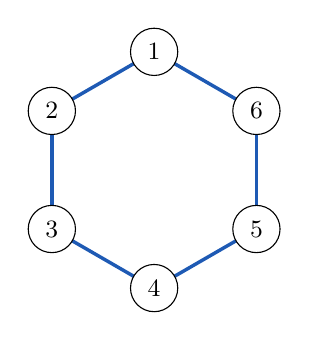
\begin{tikzpicture}[scale=1]
\coordinate (g1) at (0.0,1.5);
\coordinate (g2) at (-1.299,0.75);
\coordinate (g3) at (-1.299,-0.75);
\coordinate (g4) at (-0.0,-1.5);
\coordinate (g5) at (1.299,-0.75);
\coordinate (g6) at (1.299,0.75);
\draw[edge] (g1)--(g2);
\draw[edge] (g2)--(g3);
\draw[edge] (g3)--(g4);
\draw[edge] (g4)--(g5);
\draw[edge] (g5)--(g6);
\draw[edge] (g6)--(g1);
\node[lab] at (g1) {1};
\node[lab] at (g2) {2};
\node[lab] at (g3) {3};
\node[lab] at (g4) {4};
\node[lab] at (g5) {5};
\node[lab] at (g6) {6};
\end{tikzpicture}\end{center}\end{column}\begin{column}{.48\textwidth}In $C_6$, the sets $\{1,3,5\}$ and $\{2,4,6\}$ are independent.\par\medskip No independent set can use more than one endpoint of each of the disjoint edges $12,34,56$.\par\medskip Thus $\alpha(C_6)=3$.\par\medskip Also, $\kappa(C_6)=2$.\end{column}\end{columns}
\end{frame}

\begin{frame}{Theorem: Connectivity and Independence}
\large
\begin{block}{Theorem 1.24 (Chv\'atal--Erd\H{o}s)}
For a connected graph of order at least $3$, $\kappa(G)\ge\alpha(G)$ implies Hamiltonicity.
\end{block}
\bigskip High connectivity prevents a longest cycle from missing a component unless a large independent set exists.
\end{frame}

\begin{frame}{Proof of Theorem 1.24: Set-Up}
\large
\begin{block}{Recall}
For a connected graph of order at least $3$, $\kappa(G)\ge\alpha(G)$ implies Hamiltonicity.
\end{block}
\begin{block}{Proof}
\normalsize The hypothesis implies $\kappa(G)\ge2$: otherwise $\alpha(G)\le1$, so $G$ is complete, contradicting $\kappa(G)=1$ and $n\ge3$.\par\medskip Let $C$ be a longest cycle. If it is not spanning, choose a component $H$ of $G-V(C)$.\par\medskip Let $c_1,\ldots,c_r$ be the vertices on $C$ with neighbors in $H$, in cyclic order. Let $d_i$ be the successor of $c_i$ on the oriented cycle.
\end{block}

\end{frame}

\begin{frame}{Proof Continued: Successors of Attachment Vertices}
\large
\begin{columns}[c,onlytextwidth]\begin{column}{.48\textwidth}\begin{center}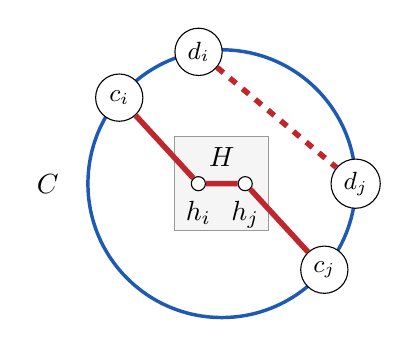
\begin{tikzpicture}[scale=.85]
\draw[edge] (0,0) circle (2);\node at (-2.6,0){$C$};
\node[lab](ci) at (140:2){$c_i$};\node[lab](di) at (100:2){$d_i$};
\node[lab](cj) at (-40:2){$c_j$};\node[lab](dj) at (0:2){$d_j$};
\draw[fill=SoftGray,draw=black!40](-.7,-.7) rectangle (.7,.7);\node at (0,.4){$H$};
\node[v,label=below:{$h_i$}](hi) at (-.35,0){};\node[v,label=below:{$h_j$}](hj) at (.35,0){};
\draw[selected](ci)--(hi)--(hj)--(cj);\draw[selected,dashed](di)--(dj);
\end{tikzpicture}\end{center}\end{column}\begin{column}{.48\textwidth}Choose $h_i\in H$ adjacent to $c_i$.\par\medskip\textbf{Observation 1.} No $d_i$ has a neighbor in $H$. Otherwise replace $c_id_i$ by a path through $H$ to obtain a longer cycle.\par\medskip\textbf{Observation 2.} Removing $c_1,\ldots,c_r$ separates $H$ from the successors on $C$. Hence $r\ge\kappa(G)$.\end{column}\end{columns}
\end{frame}

\begin{frame}{Proof Continued: The Successors Are Independent}
\large
\begin{columns}[c,onlytextwidth]\begin{column}{.48\textwidth}\begin{center}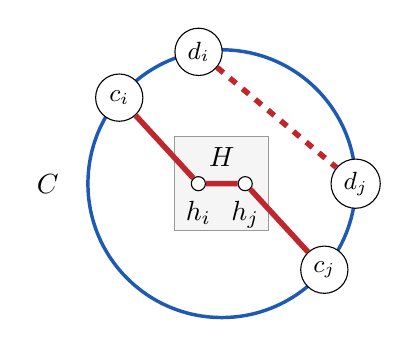
\begin{tikzpicture}[scale=.85]
\draw[edge] (0,0) circle (2);\node at (-2.6,0){$C$};
\node[lab](ci) at (140:2){$c_i$};\node[lab](di) at (100:2){$d_i$};
\node[lab](cj) at (-40:2){$c_j$};\node[lab](dj) at (0:2){$d_j$};
\draw[fill=SoftGray,draw=black!40](-.7,-.7) rectangle (.7,.7);\node at (0,.4){$H$};
\node[v,label=below:{$h_i$}](hi) at (-.35,0){};\node[v,label=below:{$h_j$}](hj) at (.35,0){};
\draw[selected](ci)--(hi)--(hj)--(cj);\draw[selected,dashed](di)--(dj);
\end{tikzpicture}\end{center}\end{column}\begin{column}{.48\textwidth}\textbf{Observation 3.} No two successors $d_i,d_j$ are adjacent.\par\medskip If they were, use a path through $H$ from $c_i$ to $c_j$, then follow $C$ backwards to $d_i$, cross to $d_j$, and follow $C$ forwards to $c_i$.\par\medskip This cycle contains all of $C$ and at least one vertex of $H$, a contradiction.\end{column}\end{columns}
\end{frame}

\begin{frame}{Proof Continued: The Contradiction}
\large
\begin{block}{Recall}
For a connected graph of order at least $3$, $\kappa(G)\ge\alpha(G)$ implies Hamiltonicity.
\end{block}
\begin{block}{Proof}
\normalsize Choose any vertex $h\in H$. The observations show that\[\{h,d_1,\ldots,d_r\}\]is independent: no two successors are adjacent, and no successor has a neighbor in $H$.\par\medskip Consequently,\[\alpha(G)\ge r+1\ge\kappa(G)+1,\]contrary to $\kappa(G)\ge\alpha(G)$. Thus the longest cycle is spanning.\hfill$\square$
\end{block}

\end{frame}

\begin{frame}{The Petersen Graph}
\large
\begin{columns}[c,onlytextwidth]\begin{column}{.48\textwidth}\begin{center}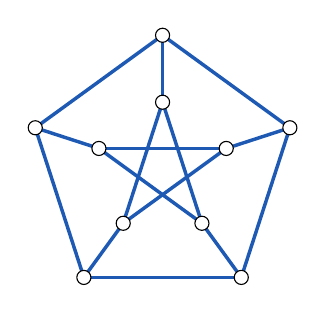
\begin{tikzpicture}[scale=0.85]
\coordinate (g1) at (0.0,2.0);
\coordinate (g2) at (-1.902,0.618);
\coordinate (g3) at (-1.176,-1.618);
\coordinate (g4) at (1.176,-1.618);
\coordinate (g5) at (1.902,0.618);
\coordinate (g6) at (0.0,1.0);
\coordinate (g7) at (-0.951,0.309);
\coordinate (g8) at (-0.588,-0.809);
\coordinate (g9) at (0.588,-0.809);
\coordinate (g10) at (0.951,0.309);
\draw[edge] (g1)--(g2);
\draw[edge] (g2)--(g3);
\draw[edge] (g3)--(g4);
\draw[edge] (g4)--(g5);
\draw[edge] (g5)--(g1);
\draw[edge] (g1)--(g6);
\draw[edge] (g2)--(g7);
\draw[edge] (g3)--(g8);
\draw[edge] (g4)--(g9);
\draw[edge] (g5)--(g10);
\draw[edge] (g6)--(g8);
\draw[edge] (g8)--(g10);
\draw[edge] (g10)--(g7);
\draw[edge] (g7)--(g9);
\draw[edge] (g9)--(g6);
\node[v] at (g1) {};
\node[v] at (g2) {};
\node[v] at (g3) {};
\node[v] at (g4) {};
\node[v] at (g5) {};
\node[v] at (g6) {};
\node[v] at (g7) {};
\node[v] at (g8) {};
\node[v] at (g9) {};
\node[v] at (g10) {};
\end{tikzpicture}\end{center}\end{column}\begin{column}{.48\textwidth}The Petersen graph has\[\kappa(G)=3,\qquad\alpha(G)=4.\]It is not Hamiltonian.\par\medskip Thus replacing $\kappa(G)\ge\alpha(G)$ by $\kappa(G)\ge\alpha(G)-1$ would not work.\par\medskip\textbf{Exercise:} find an independent set of size $4$.\end{column}\end{columns}
\end{frame}

\begin{frame}{Definition: Forbidden Induced Subgraphs}
\large
\begin{block}{$H$-free}
A graph $G$ is $H$-free if no induced subgraph of $G$ is isomorphic to $H$.
\end{block}
\begin{block}{$\mathcal S$-free}
A graph is $\mathcal S$-free if it is $H$-free for every $H\in\mathcal S$.
\end{block}
\medskip\textbf{Induced matters:} select vertices and retain every edge between them. Extra edges can prevent an induced copy.
\end{frame}

\begin{frame}{Three Important Forbidden Graphs}
\large
\begin{columns}\begin{column}{.32\textwidth}\begin{center}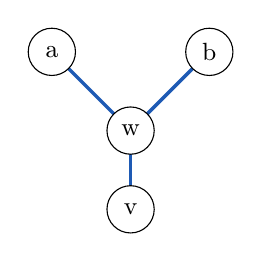
\begin{tikzpicture}[scale=1]
\coordinate (gw) at (0,0);
\coordinate (ga) at (-1,1);
\coordinate (gb) at (1,1);
\coordinate (gv) at (0,-1);
\draw[edge] (gw)--(ga);
\draw[edge] (gw)--(gb);
\draw[edge] (gw)--(gv);
\node[lab] at (gw) {w};
\node[lab] at (ga) {a};
\node[lab] at (gb) {b};
\node[lab] at (gv) {v};
\end{tikzpicture}\end{center}\begin{center}Claw: $K_{1,3}$\end{center}\end{column}\begin{column}{.32\textwidth}\begin{center}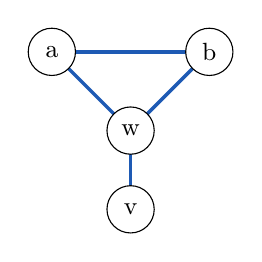
\begin{tikzpicture}[scale=1]
\coordinate (gw) at (0,0);
\coordinate (ga) at (-1,1);
\coordinate (gb) at (1,1);
\coordinate (gv) at (0,-1);
\draw[edge] (gw)--(ga);
\draw[edge] (gw)--(gb);
\draw[edge] (gw)--(gv);
\draw[edge] (ga)--(gb);
\node[lab] at (gw) {w};
\node[lab] at (ga) {a};
\node[lab] at (gb) {b};
\node[lab] at (gv) {v};
\end{tikzpicture}\end{center}\begin{center}$Z_1$: a triangle with a leaf\end{center}\end{column}\begin{column}{.32\textwidth}\begin{center}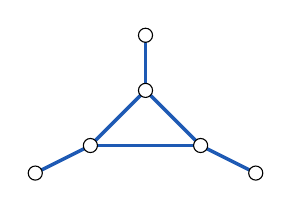
\begin{tikzpicture}[scale=0.7]
\coordinate (g1) at (0,1);
\coordinate (g2) at (-1,0);
\coordinate (g3) at (1,0);
\coordinate (g4) at (0,2);
\coordinate (g5) at (-2,-0.5);
\coordinate (g6) at (2,-0.5);
\draw[edge] (g1)--(g2);
\draw[edge] (g2)--(g3);
\draw[edge] (g3)--(g1);
\draw[edge] (g1)--(g4);
\draw[edge] (g2)--(g5);
\draw[edge] (g3)--(g6);
\node[v] at (g1) {};
\node[v] at (g2) {};
\node[v] at (g3) {};
\node[v] at (g4) {};
\node[v] at (g5) {};
\node[v] at (g6) {};
\end{tikzpicture}\end{center}\begin{center}$N$: a triangle with three leaves\end{center}\end{column}\end{columns}
\end{frame}

\begin{frame}{Theorem: Two Forbidden Subgraphs}
\large
\begin{block}{Theorem 1.25}
Every $2$-connected $\{K_{1,3},Z_1\}$-free graph is Hamiltonian.
\end{block}
\begin{columns}[c,onlytextwidth]\begin{column}{.48\textwidth}\begin{center}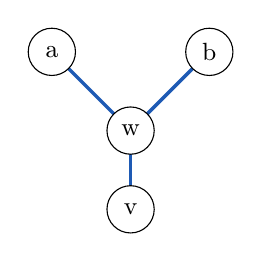
\begin{tikzpicture}[scale=1]
\coordinate (gw) at (0,0);
\coordinate (ga) at (-1,1);
\coordinate (gb) at (1,1);
\coordinate (gv) at (0,-1);
\draw[edge] (gw)--(ga);
\draw[edge] (gw)--(gb);
\draw[edge] (gw)--(gv);
\node[lab] at (gw) {w};
\node[lab] at (ga) {a};
\node[lab] at (gb) {b};
\node[lab] at (gv) {v};
\end{tikzpicture}\end{center}\end{column}\begin{column}{.48\textwidth}\begin{center}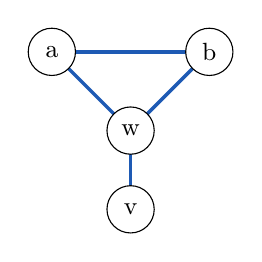
\begin{tikzpicture}[scale=1]
\coordinate (gw) at (0,0);
\coordinate (ga) at (-1,1);
\coordinate (gb) at (1,1);
\coordinate (gv) at (0,-1);
\draw[edge] (gw)--(ga);
\draw[edge] (gw)--(gb);
\draw[edge] (gw)--(gv);
\draw[edge] (ga)--(gb);
\node[lab] at (gw) {w};
\node[lab] at (ga) {a};
\node[lab] at (gb) {b};
\node[lab] at (gv) {v};
\end{tikzpicture}\end{center}\end{column}\end{columns}
\end{frame}

\begin{frame}{Proof of Theorem 1.25: A Longest Cycle}
\large
\begin{block}{Recall}
Every $2$-connected $\{K_{1,3},Z_1\}$-free graph is Hamiltonian.
\end{block}
\begin{block}{Proof}
\normalsize Let $C$ be a longest cycle. If $C$ is not spanning, connectedness gives a vertex $v\notin C$ adjacent to $w\in C$.\par\medskip Let $a,b$ be the predecessor and successor of $w$ on $C$. Neither $av$ nor $bv$ can be an edge: either would let us insert $v$ into $C$.\par\medskip We now consider whether $a$ and $b$ are adjacent.
\end{block}

\end{frame}

\begin{frame}{Proof Continued: Two Cases}
\large
\begin{columns}[c,onlytextwidth]\begin{column}{.48\textwidth}\begin{center}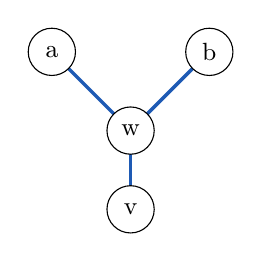
\begin{tikzpicture}[scale=1]
\coordinate (gw) at (0,0);
\coordinate (ga) at (-1,1);
\coordinate (gb) at (1,1);
\coordinate (gv) at (0,-1);
\draw[edge] (gw)--(ga);
\draw[edge] (gw)--(gb);
\draw[edge] (gw)--(gv);
\node[lab] at (gw) {w};
\node[lab] at (ga) {a};
\node[lab] at (gb) {b};
\node[lab] at (gv) {v};
\end{tikzpicture}\end{center}\begin{block}{Case 1: $ab$ is absent}
The vertices $w,a,b,v$ induce a claw.
\end{block}
\end{column}\begin{column}{.48\textwidth}\begin{center}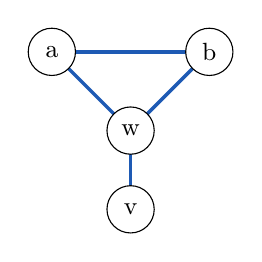
\begin{tikzpicture}[scale=1]
\coordinate (gw) at (0,0);
\coordinate (ga) at (-1,1);
\coordinate (gb) at (1,1);
\coordinate (gv) at (0,-1);
\draw[edge] (gw)--(ga);
\draw[edge] (gw)--(gb);
\draw[edge] (gw)--(gv);
\draw[edge] (ga)--(gb);
\node[lab] at (gw) {w};
\node[lab] at (ga) {a};
\node[lab] at (gb) {b};
\node[lab] at (gv) {v};
\end{tikzpicture}\end{center}\begin{block}{Case 2: $ab$ is present}
The vertices $w,a,b,v$ induce $Z_1$.
\end{block}
\end{column}\end{columns}\medskip Both cases contradict the forbidden-subgraph hypothesis.\par\smallskip Hence $C$ is Hamiltonian.\hfill$\square$
\end{frame}

\begin{frame}{Theorem: Forbidding the Claw and the Net}
\large
\begin{block}{Theorem 1.26}
For a $\{K_{1,3},N\}$-free graph $G$:\begin{enumerate}\item Connectedness implies traceability.\item $2$-connectedness implies Hamiltonicity.\end{enumerate}
\end{block}
\begin{columns}[c,onlytextwidth]\begin{column}{.48\textwidth}\begin{center}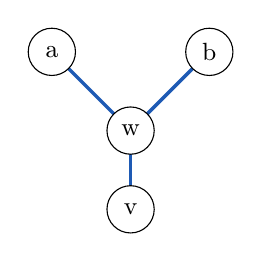
\begin{tikzpicture}[scale=1]
\coordinate (gw) at (0,0);
\coordinate (ga) at (-1,1);
\coordinate (gb) at (1,1);
\coordinate (gv) at (0,-1);
\draw[edge] (gw)--(ga);
\draw[edge] (gw)--(gb);
\draw[edge] (gw)--(gv);
\node[lab] at (gw) {w};
\node[lab] at (ga) {a};
\node[lab] at (gb) {b};
\node[lab] at (gv) {v};
\end{tikzpicture}\end{center}\end{column}\begin{column}{.48\textwidth}\begin{center}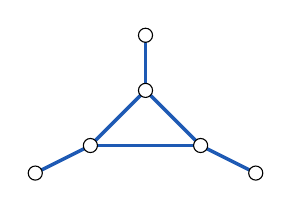
\begin{tikzpicture}[scale=0.7]
\coordinate (g1) at (0,1);
\coordinate (g2) at (-1,0);
\coordinate (g3) at (1,0);
\coordinate (g4) at (0,2);
\coordinate (g5) at (-2,-0.5);
\coordinate (g6) at (2,-0.5);
\draw[edge] (g1)--(g2);
\draw[edge] (g2)--(g3);
\draw[edge] (g3)--(g1);
\draw[edge] (g1)--(g4);
\draw[edge] (g2)--(g5);
\draw[edge] (g3)--(g6);
\node[v] at (g1) {};
\node[v] at (g2) {};
\node[v] at (g3) {};
\node[v] at (g4) {};
\node[v] at (g5) {};
\node[v] at (g6) {};
\end{tikzpicture}\end{center}\end{column}\end{columns}
\end{frame}

\section{Three Open Problems}
\begin{frame}{Three Open Problems}
\large
The final part of the section moves from theorems to conjectures.\begin{itemize}\setlength{\itemsep}{.22cm}
\item Do any three longest paths share a vertex?
\item Does $4$-connectivity force a claw-free graph to be Hamiltonian?
\item Can the vertex set always be partitioned with prescribed bounds on longest paths?
\end{itemize}\bigskip We follow the problems and numbering of Section 1.4.4.
\end{frame}

\begin{frame}{Definition: Detour Order and Detour Path}
\large
\begin{block}{Detour order}
$\tau(G)$ is the number of vertices in a longest path of $G$.
\end{block}
\begin{block}{Detour path}
A path with $\tau(G)$ vertices is called a detour path.
\end{block}
\medskip For example, $\tau(P_n)=n$, $\tau(C_n)=n$, and $\tau(K_{1,3})=3$.\par\medskip Detour order counts \textbf{vertices}, rather than edges.
\end{frame}

\begin{frame}{Any Two Longest Paths Intersect}
\large
\begin{block}{Claim}
Any two longest paths in a connected graph share a vertex.
\end{block}
\begin{block}{Proof}
\normalsize Suppose disjoint longest paths $P,Q$ each have $L$ edges. Choose a shortest path joining them, with endpoints $x\in P$ and $y\in Q$ and no internal vertex on either.\par\medskip From $x$, one half of $P$ has at least $L/2$ edges; similarly for $Q$ at $y$. Joining these two halves gives a path of length at least $L+1$, a contradiction.\hfill$\square$
\end{block}

\end{frame}

\begin{frame}{What About Three Longest Paths?}
\large
\begin{block}{Conjecture 1}
For three detour paths $P_1,P_2,P_3$ in a connected graph,\[V(P_1)\cap V(P_2)\cap V(P_3)\ne\varnothing.\]
\end{block}
\medskip Pairwise intersection alone does not imply a common vertex.\par\medskip The question asks whether being \emph{longest paths in the same graph} supplies the missing structure.
\end{frame}

\begin{frame}{All Longest Paths Need Not Share a Vertex}
\large
The analogous statement for the entire family of longest paths is false.\begin{block}{Examples discussed in the textbook}
The section gives a $12$-vertex graph with detour order $10$, and another graph with seven detour paths whose common intersection is empty.
\end{block}
\medskip These examples explain why the question about \textbf{three} paths is more delicate than the question about all paths.
\end{frame}

\begin{frame}{Two More Forbidden Graphs}
\large
\begin{columns}[c,onlytextwidth]\begin{column}{.48\textwidth}\begin{center}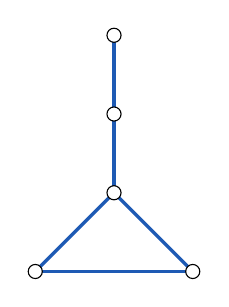
\begin{tikzpicture}[scale=1]
\coordinate (g1) at (0,0);
\coordinate (g2) at (-1,-1);
\coordinate (g3) at (1,-1);
\coordinate (g4) at (0,1);
\coordinate (g5) at (0,2);
\draw[edge] (g1)--(g2);
\draw[edge] (g2)--(g3);
\draw[edge] (g3)--(g1);
\draw[edge] (g1)--(g4);
\draw[edge] (g4)--(g5);
\node[v] at (g1) {};
\node[v] at (g2) {};
\node[v] at (g3) {};
\node[v] at (g4) {};
\node[v] at (g5) {};
\end{tikzpicture}\end{center}\begin{center}$Z_2$\end{center}\end{column}\begin{column}{.48\textwidth}\begin{center}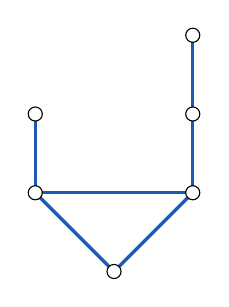
\begin{tikzpicture}[scale=1]
\coordinate (g1) at (0,-1);
\coordinate (g2) at (-1,0);
\coordinate (g3) at (1,0);
\coordinate (g4) at (-1,1);
\coordinate (g5) at (1,1);
\coordinate (g6) at (1,2);
\draw[edge] (g1)--(g2);
\draw[edge] (g2)--(g3);
\draw[edge] (g3)--(g1);
\draw[edge] (g2)--(g4);
\draw[edge] (g3)--(g5);
\draw[edge] (g5)--(g6);
\node[v] at (g1) {};
\node[v] at (g2) {};
\node[v] at (g3) {};
\node[v] at (g4) {};
\node[v] at (g5) {};
\node[v] at (g6) {};
\end{tikzpicture}\end{center}\begin{center}$W$\end{center}\end{column}\end{columns}\medskip Each starts with a triangle. In $Z_2$, attach a two-edge path at one vertex. In $W$, also attach a leaf at another triangle vertex.
\end{frame}

\begin{frame}{Why Does the Claw Keep Appearing?}
\large
\begin{block}{Theorem 1.27}
Let $R,S$ be connected graphs other than $P_3$. If forbidding $R,S$ as induced subgraphs forces every $2$-connected graph to be Hamiltonian, then one of $R,S$ is $K_{1,3}$ and the other is an induced subgraph of $P_6,Z_2,W$, or $N$.
\end{block}
\medskip The graphs $Z_2$ and $W$ are shown on the previous slide.\par\medskip The claw is an essential part of such forbidden pairs.
\end{frame}

\begin{frame}{Matthews--Sumner's Conjecture}
\large
\begin{block}{Conjecture 2}
Every $4$-connected claw-free graph is Hamiltonian.
\end{block}
\medskip $3$-connectivity is insufficient: there are $3$-connected claw-free non-Hamiltonian graphs.\begin{block}{Theorem 1.28 (as stated in the textbook)}
Every $7$-connected claw-free graph is Hamiltonian.
\end{block}
\small\medskip Later work improves the sufficient connectivity from $7$ to $6$.\par\smallskip{\tiny See Allred and Ellingham, \emph{Unavoidable induced subgraphs of large and infinite 2-edge-connected graphs}, 2026, Section 1.2.}
\end{frame}

\begin{frame}{Definition: An $(a,b)$-Partition}
\large
Write $\langle A\rangle$ for the subgraph induced by a vertex set $A$.\begin{block}{$(a,b)$-partition}
A partition $V(G)=A\sqcup B$ such that\[\tau(\langle A\rangle)\le a,\qquad\tau(\langle B\rangle)\le b.\]
\end{block}
\medskip The bounds concern longest paths within the two induced graphs. There may be many edges between $A$ and $B$.
\end{frame}

\begin{frame}{Example: Partitioning a Cycle}
\large
\begin{columns}[c,onlytextwidth]\begin{column}{.48\textwidth}\begin{center}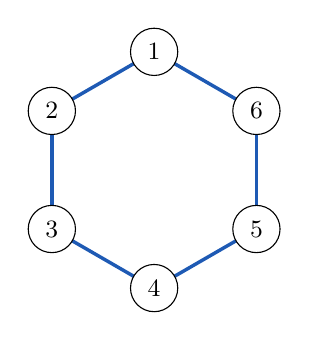
\begin{tikzpicture}[scale=1]
\coordinate (g1) at (0.0,1.5);
\coordinate (g2) at (-1.299,0.75);
\coordinate (g3) at (-1.299,-0.75);
\coordinate (g4) at (-0.0,-1.5);
\coordinate (g5) at (1.299,-0.75);
\coordinate (g6) at (1.299,0.75);
\draw[edge] (g1)--(g2);
\draw[edge] (g2)--(g3);
\draw[edge] (g3)--(g4);
\draw[edge] (g4)--(g5);
\draw[edge] (g5)--(g6);
\draw[edge] (g6)--(g1);
\node[lab] at (g1) {1};
\node[lab] at (g2) {2};
\node[lab] at (g3) {3};
\node[lab] at (g4) {4};
\node[lab] at (g5) {5};
\node[lab] at (g6) {6};
\end{tikzpicture}\end{center}\end{column}\begin{column}{.48\textwidth}Here $\tau(C_6)=6$.\par\medskip Let $A=\{1,3,5\}$ and $B=\{2,4,6\}$. Both induced graphs have no edges, so both have detour order $1$.\par\medskip This is a valid $(a,b)$-partition for every positive $a,b$ with $a+b=6$.\end{column}\end{columns}
\end{frame}

\begin{frame}{The Path Partition Conjecture}
\large
\begin{block}{$\tau$-partitionable}
$G$ is $\tau$-partitionable if it has an $(a,b)$-partition for every pair of positive integers satisfying $a+b=\tau(G)$.
\end{block}
\begin{block}{Path Partition Conjecture}
Every graph is $\tau$-partitionable.
\end{block}
\medskip The partition may depend on $(a,b)$.\par\smallskip One fixed partition need not work for every pair.
\end{frame}

\begin{frame}{Known Cases of the Path Partition Conjecture}
\large
\begin{block}{Theorem 1.29}
$G$ is $\tau$-partitionable if any of these conditions holds:\begin{enumerate}\item $\Delta(G)\le3$;\item $\Delta(G)\ge |V(G)|-8$;\item $\tau(G)\le13$;\item $\tau(G)\ge |V(G)|-1$.\end{enumerate}
\end{block}
\medskip These are the sufficient conditions listed in the textbook.
\end{frame}

\begin{frame}{The Claw Appears Again}
\large
\begin{block}{Theorem 1.30}
Every claw-free graph is $\tau$-partitionable.
\end{block}
\begin{center}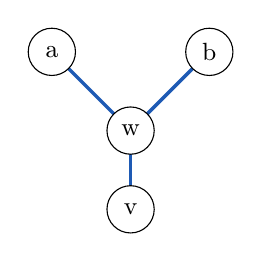
\begin{tikzpicture}[scale=1]
\coordinate (gw) at (0,0);
\coordinate (ga) at (-1,1);
\coordinate (gb) at (1,1);
\coordinate (gv) at (0,-1);
\draw[edge] (gw)--(ga);
\draw[edge] (gw)--(gb);
\draw[edge] (gw)--(gv);
\node[lab] at (gw) {w};
\node[lab] at (ga) {a};
\node[lab] at (gb) {b};
\node[lab] at (gv) {v};
\end{tikzpicture}\end{center}\medskip The same small forbidden graph appears in both Hamiltonicity and path-partition results.
\end{frame}

\begin{frame}{Summary: Trails, Circuits, Paths, and Cycles}
\large
\begin{itemize}\setlength{\itemsep}{.22cm}
\item \textbf{Eulerian routes:} use every edge; degree parity gives a complete criterion.
\item \textbf{Finding circuits:} Hierholzer\textquotesingle s algorithm joins circuits along shared vertices.
\item \textbf{Hamiltonian routes:} visit every vertex; degree bounds, connectivity, and forbidden induced subgraphs give sufficient conditions.
\item \textbf{Further questions:} intersecting longest paths, claw-free Hamiltonicity, and path partitions.
\end{itemize}
\end{frame}

\begin{frame}{Next time: Planarity}
\large
\begin{center}{\Huge Planarity}\end{center}
\end{frame}
\end{document}